\chapter{Introduction to Elliptic Curves} \label{Ch:EllipticCurve}
\section{Mathematical Foundations}
\subsection*{Finite Groups}
A Finite Group is a set G with a finite number of $q$ elements, which has a binary operation $*$ : $G * G \rightarrow G$ and satisfies the following properties \cite{hankerson2006guide}:
\begin{enumerate}
	\item Associativity: $(a*b)*c=a*(b*c)$ for all elements $a,b,c \in G$
	\item Existence of an identity: there exists an element $e \in G$ such that $a*e=e*a=a$ for all $a \in G$. Element $e$ is called the neutral element (or identity element) of the group.
	\item Existence of inverses: for each element $a \in G$, there exists an element $b \in G$ such that $a*b=b*a=e$. Element $b$ is called the inverse of $a$.
\end{enumerate}
$q$ is called the group order. In addition, a group is called Abelian group (or commutative group) if it satisfies the commutativity law which is $a*b=b*a$ for all elements $a,b \in G$. 

If the binary operation is called addition (+), then the group is additive. In this case, the neutral element is usually denoted by 0 and the additive inverse of an element $a$ is denoted by $-a$. If the binary operation is called multiplication $(\cdot)$, then the finite group is multiplicative. In this case, the identity element is usually denoted by 1 and the multiplicative inverse of an element $a$ is denoted by $a^{-1}$.

\subsection*{Finite Fields}
Abstractly, a finite field consists of a finite set of objects called field elements together with the description of two operations, addition and multiplication, that can be performed on pairs of field elements. These operations must have certain properties: \cite{hankerson2006guide}
\begin{enumerate}
	\item $(\mathbb{F},+)$ is an Abelian group with (additive) neutral element denoted by 0.
	\item $(\mathbb{F},\cdot)$ is an Abelian group with (multiplicative) neutral element denoted by 1.
	\item The distributive law holds: $(a+b) \cdot c = a \cdot c + b \cdot c$ for all $a,b,c \in \mathbb{F}$. 
\end{enumerate}

\paragraph{Prime Fields}\mbox{}\\
Let $p$ be a prime number. The residues modulo $p$, consisting of the integers $\left\lbrace 0,1,2,\dots,p-1\right\rbrace $ with addition and multiplication performed modulo $p$, is a finite field of order $p$.
\paragraph{Binary Fields}\mbox{}\\
Finite fields of order $2^m$ are called binary fields or characteristic-two finite fields. One way to construct $\mathbb{F}_{2^m}$ is to use a polynomial basis representation. The elements of $\mathbb{F}_{2^m}$ are the binary polynomials (polynomials whose coefficients are in the field $\mathbb{F}_2=\{0,1\}$) of degree at most $m-1$:
$$\mathbb{F}_{2^m}=\left\lbrace a_{m-1}z^{m-1}+\dots+a_2z^2+a_1z^1+a_0 : a_i \in \mathbb{F}_2 ;+, \cdot \right\rbrace. $$
An irreducible binary polynomial $f(z)$ of degree m is chosen. Irreducibility of $f(z)$ means that $f(z)$ cannot be factored as a product of binary polynomials each of degree less than $m$. Addition of field elements is the usual addition of polynomials, with coefficient reduced modulo 2. Multiplication of field elements is performed as multiplication of polynomials modulo the polynomial $f(z)$. 
\subsection*{Cyclic Groups}
Let $G$ be a finite group of order $q$ with multiplication ($\cdot$) as binary operation, $g$ be a group element of $G$, then the order of $g$ is the smallest positive integer $r$ for which $g^r = 1$.  
$G$ is called cyclic if there exist a $g$ such that $\langle g \rangle = \left\lbrace g^i : 0 \leq i \leq r-1 \right\rbrace $ is the subgroup of $G$ generated by $g$. If $r=q$ then $G$ is a cyclic group with generator $g$ if $G = \langle g \rangle$. The set $\langle
 g \rangle$ is also a group itself under the same binary operation and is called the cyclic subgroup of $G$ generated by $g$.
 
%\subsection{Generalized discrete logarithm problem}
%Given a multiplicative cyclic group $(G,\cdot)$ of order n with generator g and an element $y \in \

\section{Elliptic Curves} \label{sec:EC}
An elliptic curve over a field $K$ is defined by a set of points which satisfy the following equation (also known as standard Weierstrass form) and a group operation which will be defined later.
\begin{equation} \label{eq:ECWeierstrass}
y^3+a_1xy+a_3y = x^3 + a_2x^2+a_4x+a_6
\end{equation}

Here: $a_1,a_2,a_3,a_4,a_6 \in K$, and the discriminant is defined as
 $$\Delta=-d^{2}_{2}d_{8}-8d_{4}^{3}-27d_{6}^{2}+9d_{2}d_{4}d_{6} \neq 0$$
where  
$$d_{2}=a_{1}^{2}+4a_{2}$$  $$d_{4}=2a_{4}+a_1a_3$$  $$d_6=a_{3}^{2}+4a_6$$  $$d_8=a_{1}^{2}a_6+4a_2a_6-a_1a_3a_4+a_2a_{3}^{2}-a_{4}^{2}$$

The condition $\Delta \neq 0$ guarantees that there does not exist more than one tangent line for a given point on the curve.

For an elliptic curve over a field K of characteristic $\neq$ 2 or 3, without loss of generality, one can assume that $a_1=a_2=a_3=0$, we have $d_2=0$, $d_4=2a_4$, $d_6 = 4a_6$ and $d_8=-a_{4}^{2}$ \cite{hankerson2006guide}. Accordingly, the condition $\Delta = -16(4a_4^3+27a_6^2) \neq 0$ can be simplified to $4a_4^3+27a_6^2 \neq 0$. Consequently in practical application of elliptic curves, the curve equation is written in the following form:

\begin{equation} \label{eq:ECFp}
y^3=x^3+ax+b
\end{equation}

where $a=a_4$ and $b=a_6$, cf. Equation \ref{eq:ECWeierstrass}.

For an elliptic curve over binary fields $\mathbb{F}_2^m$, without loss of generality, one can assume that $a_1=1$, $a_3=a_4=0$ \cite{hankerson2006guide}. Then we have $d_2=1$, $d_4=0$, $d_6=0$ and $d_8=a_6$ \footnote{In binary fields anything multiplied by 2 equals to 0.}, and $\Delta = -a_6 \neq 0$. The short form of curve equation is normally written as follows: 
\begin{equation}\label{eq:ECF2m}
y^2+xy=x^3+ax^2+b
\end{equation}

where $ a = a_2$ and $b = a_6$ and $a,b \in \mathbb{F}_2^m$. 
%\cite{koblitz1987elliptic}

\subsection{Elliptic Curves Over $\mathbb{F}_p$}
The finite field $\mathbb{F}_p$ uses the numbers from 0 to $p-1$, and computations are done modulo $p$. An Elliptic Curve over finite field $\mathbb{F}_p$ where $p$ is a large prime, can be formed by choosing the constants $a$ and $b$ within the field $\mathbb{F}_p$. The elliptic curve includes all points $(x,y)$ which satisfy the elliptic curve equation modulo $p$ (where x and y are numbers in $\mathbb{F}_p$). It is typically defined in the short Weierstrass form:
$$y^2 \text{ mod } p= x^3 + ax + b \text{ mod } p$$

where $a,b \in \mathbb{F}_p$ satisfy $4a^3 + 27b^2 \text{ mod }p$ is not 0, which guarantees $x^3 + ax + b$ contains no repeated factors and then the elliptic curve is a group. The elliptic curve contains all points $P = (x,y)$ for $x,y \in F_p$ that satisfy the elliptic curve equation with addition of (for Weierstrass curves) a special point $\mathcal{O}$ called the point at infinity \footnote{In code implementation, $\mathcal{O}$ is normally be represented as point (0,0), but not always, as (0,0) might satisfy the curve equation.}.   
    
To give an example, consider an elliptic curve over the field $F_{19}$, where $a=1$ and $b=6$, the curve equation is: $y^2 = x^3 + x + 6$, an example used in \cite{balasubramanian1998improbability}. There are 18 points: 
\begin{center}
 $ (0,5)$, $(4,6)$, $(2,4)$, $(3,6)$, $(14,3)$, $(12,13)$, \\
$ (18,2)$, $(10,3)$, $(6,0)$, $(10,16)$, $(18,17)$, $(12,16)$, \\
$ (14,16)$, $(3,13)$, $(2,15)$, $(4,13)$, $(0,14)$, $\mathcal{O}$ 
\end{center}
The point $P=(4,6)$ satisfies this equation since:
\begin{center}
$ 6^2 \mod{19} = 4^3 + 4 + 6 \mod{19} $\\
$ 17 = 17 $ 
\end{center}
\textbf{Remark:} In mod $p$ Weierstrass curves $-(x,y) = (x,-y)$

\subsection{Binary Elliptic Curves}
Elements of the field $\mathbb{F}_{2^m}$ are m-bit strings. The rules for arithmetic in binary field can be defined by either polynomial basis or by so-called (more efficient) [optimal] normal basis\cite{IEEEP1363}. An elliptic curve $E$ with the underlying field $\mathbb{F}_{2^m}$ is given through the following equation: $$y^2+xy=x^3+ax^2+b$$ where $x,y,a,b \in \mathbb{F}_{2^m}$ and $b \neq 0$. The elliptic curve $E$ includes all points $(x,y)$ which satisfy the curve equation over $\mathbb{F}_{2^m}$, together with a point at infinity $\mathcal{O}$. 

To given an example, assume the finite field $\mathbb{F}_{2^4}$ has irreducible polynomial $f(x)=x^4+x+1$ (or $\mathtt{0x13}$ in hex). The element $g = (0010)$ is a generator for the field. The powers of g are:
%{small eq1 eq2}
\begin{small}
$$g^0=(0001), g^1=(0010), g^2=(0100), g^3=(1000), g^4=(0011),g^5=(0110)$$
$$g^6=(1100), g^7=(1011), g^8=(0101), g^9=(1010), g^{10}=(0111),g^{11}=(1110)$$
$$g^{12}=(1111), g^{13}=(1101), g^{14}=(1001), g^{15}=(0001)$$
\end{small}
%put somewher I have developed a lab for UCL  in which student can benchmark field operations, SCA etc 
%low level c/c++ programming
Consider the elliptic curve $y^2+xy=x^3+g^4x^2+1$. The points on $E$ are the following and shown in Figure \ref{fig:ecc_gf2m_example}.
\begin{small}
$$(1,g^{13}), (g^3,g^{13}) ,(g^5,g^{11}),(g^6,g^{14}),(g^9,g^{13}),(g^{10},g^8),(g^{12},g^{12}),$$
$$(1,g^6),(g^3,g^8),(g^5,g^3),(g^6,g^8),(g^9,g^{10}),(g^{10},g),(g^{12},0),(0,1), \mathcal{O}$$
\end{small}
    \begin{figure}[h!]
    	\centering
    	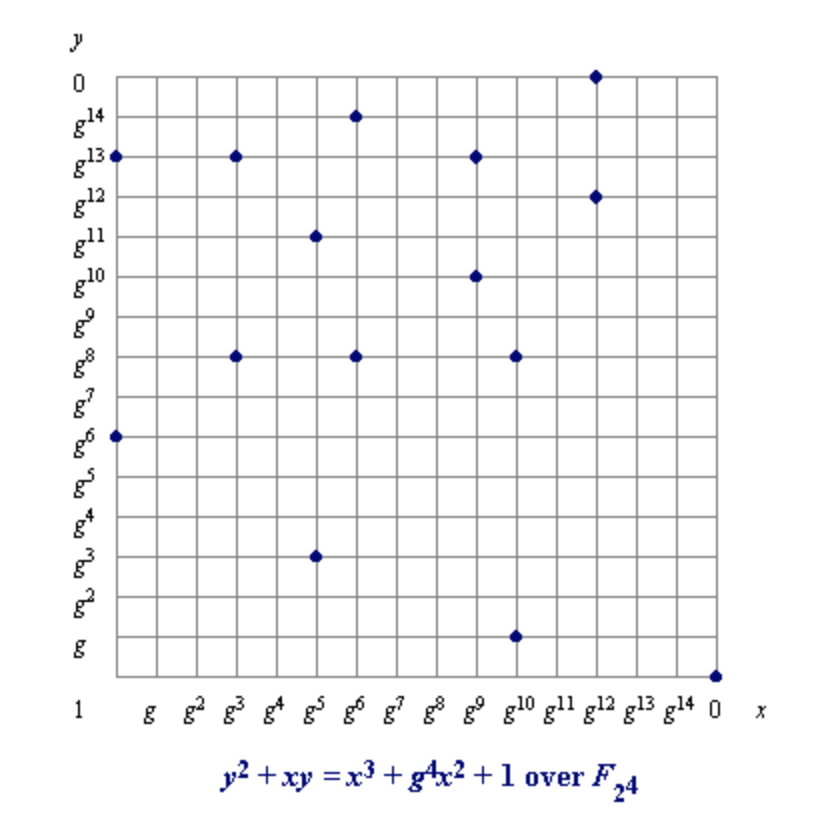
\includegraphics[width=100mm]{./pics/example_of_gf2m.png}
    	\caption{Example of elliptic curve over $\mathbb{F}_{2^4}$ }
    	\label{fig:ecc_gf2m_example}
    \end{figure}
    
\section{Point Arithmetic}
\subsection*{Point Addition for Prime Curves}
Let $P$ and $Q$ be two distinct points on an elliptic curve, and $P$ not equals to $-Q$. To add the points $P$ and $Q$, a line \footnote{line is a set of points which satisfy the equation $Ax+By+C = 0$ where $A,B,C \in \mathbb{F}_p$} is drawn through the two points. This line will have exactly one additional intersection point with the elliptic curve, which we call $-R$. The point $-R$ is ``reflected" in the x-axis to obtain point $R$. The law for point addition in an elliptic curve group is $P+Q=R$.  An example of geometrical graph is given in Figure \ref{fig:ecc_point_addition}. 
    \begin{figure}[h!]
    	\centering
    	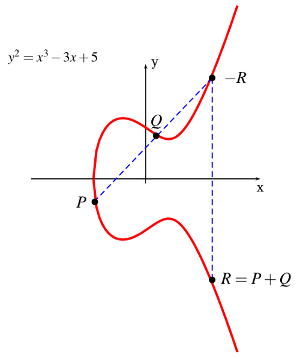
\includegraphics[width=65mm]{./pics/ecc_point_addition.png}
    	\caption{Elliptic curve point addition}
    	\label{fig:ecc_point_addition}
    \end{figure}
    
For point addition of $P$ and $-P$, the line through $P$ and $-P$ is a vertical line which does not intersect the elliptic curve at a third point. Thus the point $P$ and $-P$ cannot be added using the above method. In this case we define $P + (-P) = \mathcal{O}$. 

\subsection*{Point Doubling for Prime Curves}
Adding a point $P(x,y)$ to itself, a so-called tangent line to the curve is drawn at point $P$. If y is not zero, then the tangent line has exact one intersection with the curve at point $-Q$. $-Q$ is reflected in the x-axis to point $Q$. This operation is called doubling the point $P$, and the law for doubling is the following (also shown in Figure \ref{fig:ecc_point_doubling}): 
$$P+P=2P=Q$$ 

    \begin{figure}[h!]
    	\centering
    	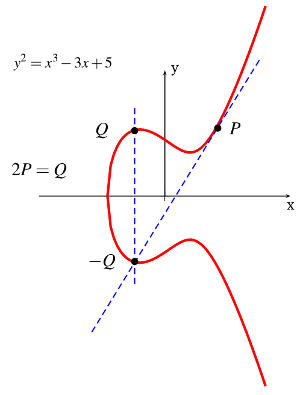
\includegraphics[width=65mm]{./pics/ecc_point_doubling.png}
    	\caption{Elliptic curve point doubling}
    	\label{fig:ecc_point_doubling}
    \end{figure}
    
Doubling the point $P(x,y)$ while $ y=0 $ then the tangent line to the curve is vertical and does not intersect the curve on any other point. For such a $P$, by definition, $2P=\mathcal{O}$, and $3P$ in this case, is $2P+P = \mathcal{O} + P = P$.   

\subsection*{Explicit Formulas for Prime Curves} \label{sec:affine_formulas}
For elliptic curves over $\mathbb{F}_p$, consider two points $P=(x_1,y_1)$ and $Q=(x_2,y_2)$, $P \neq \pm Q$, the point $P+Q = (x_3,y_3)$ is given by:
$$\lambda = \frac{y_2-y_1}{x_2-x_1}$$
$$x_3=\lambda^2-x_1-x_2$$
$$y_3=\lambda(x_1-x_3)-y_1$$

When $P=-Q$, $P+Q$ equals point at infinity $\mathcal{O}$. When $P=Q$, we apply the doubling formula:
$$\lambda = \frac{3x_1^2+a}{2y_1}$$
$$x_3=\lambda^2-2x_1$$
$$y_3=\lambda(x_1-x_3)-y_1$$



\subsection*{Scalar Multiplication}
Given an elliptic curve $E$ defined over a finite field $\mathbb{F}_p$, if $P \in E$ is a point of order $r$, the cyclic subgroup of $E$ generated by $P$ is ${\mathcal{O},P,2P,\ldots,(r-1)P}$. Then if we define the scalar $k$ as an integer within the range $[1,r-1]$, we can multiply a point by the scalar $k$ and we obtain: $Q=kP$, where $Q$ is also a point which belongs to the subgroup generated by $P$. 

\section{ECDLP}
The hardness of cryptosystem using elliptic curve point multiplication is based on the Elliptic Curve Discrete Logarithm Problem, which is an adaptation of traditional discrete logarithm problem to elliptic curves.

\begin{mydef}
Elliptic Curve Discrete Logarithm Problem (ECDLP): Given an elliptic curve $E$ defined over a finite field and two points $P,Q \in E$, find an integer $k$ such that $Q = kP$ if such $k$ exists.
\end{mydef}

The ECDLP is believed to be harder to solve than other recognized problems such as integer factorization and the discrete logarithm problem in the multiplicative group of a finite field, which are the foundations of RSA \cite{rivest1978method} and the ElGamal \cite{elgamal1985public} cryptosystems. ``Harder to solve" implies shorter keys are needed to provide the same level of security as recommended by \cite{barker2006recommendation}. Table \ref{tab:nist key length} shows the key size comparison for elliptic curves and RSA.  

\begin{table}[!h]
	\centering

	\caption{NIST's recommendation for practical applications revision 4 \cite{NSA16key}}
	\label{tab:nist key length}
	\begin{tabular}{|c|c|c|c|c|}
		\hline
		Security level in bits & Block cipher & $\mathbb{F}_p$  & $\mathbb{F}_2^m$ & RSA   \\ \hline
	\cellcolor{red}	80                     & \cellcolor{red}	SKIPJACK     & \cellcolor{red}	192 & \cellcolor{red}	163 &\cellcolor{red}	 1024  \\ \hline
		112                    & Triple-DES   & 224 & 233 & \cellcolor{orange}  2048  \\ \hline
		128                    & \cellcolor{orange} AES Small    & \cellcolor{orange}  256 & 283 & 3072  \\ \hline
		192                    & AES Medium   & 384 & 409 & \cellcolor{yellow} 7680  \\ \hline
		256                    & AES Large    & 521 & 571 & \cellcolor{yellow} 15360 \\ \hline
	\end{tabular}
\end{table}

\textbf{REMARK}: In Jan 2016, NSA has updated this table. Key changes are \cite{NSA16key}: security level less than 112 (shaded in red) are no longer approved for applying cryptographic protection on Federal government information. Algorithms (shaded in yellow) are not included in the NIST standards for interoperability and efficiency reasons. At the same time NSA announced changes from Suite B cryptography to the Commercial National Security Algorithm Suite which no longer recommends algorithms shaded in orange for national security systems \cite{NSA16}.

Common methods for solving ECDLP are Pollard’s rho algorithm and index-calculus method. We refer reader to \cite{hankerson2006guide,petit2016algebraic} for more details.
\section{An Interesting Research Question - Semaev Cipher}
When we cryptanalyse a block cipher, we write algebraic equations. Is it possible to also describe ECDLP and other EC cryptography problems by simple polynomial equations mod $p$?
\subsection{Summation Polynomials} \label{sec:summationPoly} 
Let $E$ be a general elliptic curve over field $\mathbb{F}$ in Weierstrass form given by the Equation \ref{eq:ECWeierstrass} we define $$ S_{2}\left( X_1,X_2\right)  = X_1-X_2 \in F\left[ X_1,X_2 \right] $$ The third summation polynomial to be the polynomial $S_{3}\left( X_1,X_2,X_3\right)  \in F \left[ X_1,X_2,X_3\right]$ of degree 4 by  \cite{kosters2015notes}: 
\begin{small}
	\begin{multline}\label{eq:general_Semaev}
	S_{3}\left( X_1,X_2,X_3 \right) =\left( X_1^2X_2^2+X_1^2X_3^2+X_2^2X_3^2\right) - 2\left( X_1^2X_2X_3+X_1X_2^2X_3+X_1X_2X_3^2\right)\\
	-d_2\left(X_1X_2X_3 \right) -d_4\left(X_1X_2+X_1X_3+X_2X_3 \right) -d_6\left( X_1+X_2+X_3\right) -d_8
	\end{multline}
\end{small}
then for $m \geq 4 $ in any case: \\
\begin{small}
$$S_m(X_1,\dots,X_m)=\text{Res}_X\left( S_{m-r}\left(X_1,\dots, X_{m-r-1},X \right), S_{r+2}(X_{m-r}\left( X_{m-r},\dots,X_m,X\right)  \right) $$
\end{small}
where $1 \leq r \leq m-3$.

Summation Polynomials were first introduced by Semaev in 2004 \cite{semaev2004summation}. Semaev's summation polynomials have the property that if $S_m(a_1,\dots,a_m) = 0 $ for some field elements $a_1,\dots,a_m \in F$ if and only if there are elliptic curve points $\left( a_1, b_1\right), \dots,\left( a_m,b_m \right) $ on $E$ such that $\left( a_1, b_1\right)+ \dots + \left( a_m, b_m\right) = 0 $. The idea is to represent point addition in elliptic curves using a multivariate equation system and try to solve the equation system. This topic has been studied by a lot of researchers trying to solve the ECDLP problem \cite{diem2011discrete,gaudry2004index,faugere2014using,faugere2012improving,petit2012polynomial,huang2013improvement}. In 2015 a new method was introduced by Semaev \cite{cryptoeprint:2015:310} and the idea is trying to solve the equation system by introducing new variables that lower the degree of the system of equations. In this section we will look at Semaev's summation polynomials $S_3\left( X_1,X_2,X_3\right) $ for curves over $\mathbb{F}_p$ and $\mathbb{F}_2^m$, then introduce some open research questions.  

\paragraph{Elliptic Curves Over $\mathbb{F}_p$} \mbox{} \\
For an elliptic curve over a field $K$ of characteristic $> 3$ we recall the curve equation \ref{eq:ECFp}
$y^3=x^3+a_4x+a_6$ and $S_3\left( X_1,X_2,X_3\right) $ equation can be simplified to: \cite{kosters2015notes} 

\begin{equation} \label{eq:fpCurveS3}
\begin{split}
S_3( X_1,X_2,X_3) &=( X_1^2X_2^2+X_1^2X_3^2+X_2^2X_3^2)- 2( X_1^2X_2X_3+X_1X_2^2X_3+X_1X_2X_3^2) \\
&\text{\space \space \space } -2a_4(X_1X_2+X_1X_3+X_2X_3 ) -4a_6( X_1+X_2+X_3) +a_4^2 \\
&= ( X_1-X_2)^2X_3^2-2( ( X_1X_2+a_4)(X_1+X_2 ) + 2a_6) X_3 + \left(X_1X_2-a_4 \right) ^2 \\
&\text{\space \space \space } - 4a_6(X_1+X_2)
\end{split}
\end{equation}

and it is also easy to get for point doubling when $X_1=X_2$ we have \\
\begin{equation} \label{eq:fpCurveS3Double}
-2\left( X_1^3 + 2a_4X_1+2a_6\right)X_3+\left( X_1^2 - a_4 \right)^2 - 8a_6X_1 = 0
\end{equation}
\paragraph{Special Curve secp256k1} \mbox{ } \\
For curve secp256k1 \footnote{Elliptic curve used in bitcoin; we will give more details in Section \ref{sec:seckp256k1} } where $a_4 = 0$ and $a_6 = 7$, equation \ref{eq:fpCurveS3} and equation \ref{eq:fpCurveS3Double} can be written as the following:

\begin{equation} \label{eq:secp256CurveS3}
\begin{split}
S_3( X_1,X_2,X_3) &= ( X_1-X_2)^2X_3^2-2( ( X_1X_2)(X_1+X_2 ) + 14) X_3 + X_1^2X_2^2 \\
&\text{\space \space \space } - 28(X_1+X_2)
\end{split}
\end{equation}
and for point doubling when $X_1=X_2$
$$ -2\left( X_1^3 + 14\right)X_3+ X_1^4 - 56 X_1 = 0 $$
$$ X_3 = \frac{X_1^4-56X_1}{2X_1^3+28}$$

\paragraph{Elliptic Curves Over $\mathbb{F}_{2^m}$} \mbox{} \\
For an elliptic curve over a $\mathbb{F}_2^m$, we have curve equation $y^2+xy=x^3+a_2x^2+a_6$
We have $d_2=1$, $d_4=0$, $d_6=0$ and $d_8=a_6$ (see Section \ref{sec:EC}). In binary field anything multiply by 2 equal to 0, $A-B=A+B$, thus equation \ref{eq:general_Semaev} can be simplified to:
$$S_3(X_1,X_2,X_3) = (X_1^2X_2^2+X_1^2X_3^2+X_2^2X_3^2)-X_1X_2X_3-a_6$$
$$\text{\space\space\space\space\space\space\space\space\space\space\space\space\space\space\space\space\space\space\space\space\space\space\space\space\space\space} = \left( X_1X_2+X_1X_3+X_2X_3 \right) ^2 + X_1X_2X_3+a_6$$
and when $X_1=X_2$ we have:
$$X_1^4+X_1^2X_3+a_6=0$$
$$X_3=X_1^2+\frac{a_6}{X_1^2}$$

Research question: What is the hardness of solving summation polynomials? Is it possible to solve (or improve solving) summation polynomials with similar algebraic techniques we described in previous chapters?

\subsection{Solving Semaev Equations with Extra Variables} \label{sec:SemaevCipher}
In Section \ref{sec:summationPoly} we explained the Semaev polynomials which have equations in very large degree. An interesting idea which is also used in algebraic cryptanalysis is to reduce the degree by adding new variables.
In Semaev's recent paper \cite{cryptoeprint:2015:310} he introduced a new algorithm trying to solving ECDLP using summation polynomials for curves over $F_{2^m}$. By recursively computing summation polynomials, instead of trying to write $R=P_1+\cdots+P_m$ for point $P_i$, we can write $Q_1 = P_1+P_2, Q_2=Q_1+P_3, \dots , R = Q_{m-2}+P_m$, where the $Q_i$ are completely arbitrary points (see equation \ref{eq:SemaevCipher}). Then solve the multivariate equation system under some assumptions. 
\begin{equation}
\label{eq:SemaevCipher}
\begin{cases}
S_3(Q_1,P_1,P_2) = 0 \cr
S_3(Q_1,Q_2,P_3) = 0 \cr
S_3(Q_2,Q_3,P_4) = 0 \cr
\vdots \cr
S_3(Q_i,Q_{i+1},P_{i+2}) = 0 \cr
\vdots \cr
S_3(Q_{m-2},P_m,R) = 0.
\cr
\end{cases}
\end{equation}
From this one can hope to do point splitting and index-calculus. We refer reader to \cite{cryptoeprint:2016:704,petit2016algebraic} to see how ECDLP might be solved if one can solve such equation efficiently.

However the final result of Semaev's new work is still uncertain. Some researchers believes the complexity analysis in Semaev's paper are not quite correct, cf. later work by Kosters and Yeo \cite{kosters2015notes} and blog posts \cite{StevenECDLP2015,CourtoisECCPost2015}. This leads to some open research questions. 

\paragraph{Semaev Cipher} \mbox{} \\ 
The new equation system introduced in Semaev's new paper has clear \textbf{block cipher topology} (see Figure \ref{fig:blockciphertopology} in Section \ref{sec:AA}) \cite{courtois2002cryptanalysis}. It is very similar to the block cipher equations we have tried to solve for GOST and SIMON \cite{courtois2012contradiction,courtois2014combined}. It is potentially able to be solved by methods used in algebraic cryptanalysis \cite{courtois2002cryptanalysis}. We call Semaev's new summation polynomial equations \textbf{Semaev cipher}.

It is possible to see that solving such equations can be done by similar algebraic techniques to those we studied in this thesis, and hardness of all these problems is closely related.  

%EC over F_p (point doubling in F_p summation poly)
%cost of dividing by 2 with summation polynomials for bitcoin EC


\section{Elliptic Curve in Cryptography}
Elliptic curve cryptography (ECC) was independently proposed by Neal Koblitz\cite{koblitz1987elliptic} and Victor Miller \cite{miller1985use} in 1985. It is a public-key cryptography protocol where each of the participant has a pair of keys. One private key which is kept as a secret by the owner and one public key which is public potentially for everyone. In the past 10+ years ECC has been increasingly used in practice since its inclusion in standards by organisations such as ISO, IEEE, NIST,etc. Elliptic curves are more efficient \cite{bernstein2009ebacs} and offer smaller key sizes \cite{lenstra2001selecting} at the same security as other widely adopted public key cryptography schemes such as RSA \cite{rivest1978method}. 

There are many widely used elliptic curve cryptographic schemes such as Elliptic Curve Diffie–Hellman (ECDH) key agreement scheme based on the Diffie–Hellman scheme, Elliptic Curve Integrated Encryption Scheme (ECIES), and Elliptic Curve Digital Signature Algorithm (ECDSA) etc. In this thesis we only focus on ECDSA \cite{johnson2001elliptic} (key generation part in particular) which is used in Bitcoin and we refer the readers to \cite{hankerson2006guide} for details of other schemes.

In Section \ref{domainParameters} we will describe elliptic curve domain parameters, and in Section \ref{secKeyPairGen} we will discuss elliptic curve key pair generation process, and briefly introduce ECDSA in Section \ref{sec:ecdsa}.

\subsection{Domain Parameters} \label{domainParameters}
Elliptic curve cryptographic schemes need to agree on a fixed elliptic curve and a finite field. The fixed elliptic curves are normally chosen from curves which are suggested by standard organisations, such as ISO, IEEE etc. Domain parameters for an elliptic curve scheme describe an elliptic curve $E$ defined over a finite field $\mathbb{F}_p$, a base point $G \in E\left( \mathbb{F}_p \right) $, and its order n. The parameters should be chosen so that the ECDLP is resistant to all known attacks. Domain parameters are defined as the following $D=(p,\text{FR},S,a,b,G,n,h)$ where
\begin{small}
\begin{enumerate}
	\item p is the field order
	\item FR (field representation) is an indication of the representation used for the elements of $\mathbb{F}_p$
	\item If the curve is deterministically generated, S is the seed used to generated the curve
	\item $a,b \in \mathbb{F}_p$ that define the curve equation over field $\mathbb{F}_p$
	\item $G$ is the base point where $G = \left( G_x,G_y \right) \in E(\mathbb{F}_p)$
	\item The order $n$ of $G$
	\item The cofactor $h = \frac{\#E(\mathbb{F}_p) }{n}$
\end{enumerate}
\end{small}
An example can be found in Section \ref{sec:seckp256k1}.
\subsection{Key Pair Generation}\label{secKeyPairGen}
An elliptic curve key pair is defined for a particular set of valid domain parameters (cf. \cite{hankerson2006guide} page 180 for generating and verify EC domain parameters). The public key is a random generated point $Q$ in the group $\left\langle G \right\rangle $ generated by G. The corresponding private key is $d = \log_GQ$. The key pair generation algorithm is the following:
 
\begin{algorithm}[H]
Input: Domain parameters $D=(p,FR,S,a,b,G,n,h)$ \\
Output: Public key $Q$, private key $d$ 
\caption{Key pair generation \cite{hankerson2006guide} page 180}
 \label{al:ECKey_gen}
 \begin{algorithmic} [1]
	\STATE Select $d \in _R \left[ 1, n-1 \right] $.
	\STATE Compute $Q = dG$.
	\STATE Return ($Q,d$).
 \end{algorithmic}
\end{algorithm}
Note that the process of computing a private key $d$ given public key $Q$ is exactly the elliptic curve discrete logarithm problem. Hence it is very import to chose a set of domain parameters so that the ECDLP is hard to solve. In addition the number $d$ should be \textbf{random} in the sense that the probability of any particular value being selected must be sufficiently small to prevent an adversary from gaining advantage through optimizing a search strategy based on such a probability. 

Not all the key pairs are valid keys. A public key $Q=(Q_x,Q_y)$ is valid if it satisfies all the following requirements:
\begin{enumerate}
	\item $Q \neq \mathcal{O}$ ( $\mathcal{O}$ is the point at infinity).
	\item $Q_x$ and $Q_y$ are properly represented elements of $\mathbb{F}_p$ (i.e., integers in [$0,p-1$] for prime field and bit strings of length m for binary field $\mathbb{F}_2^m$).
	\item $Q$ satisfies the elliptic curve equation defined by $a$ and $b$.
	\item we can also verify that $nQ=\mathcal{O}$.
\end{enumerate}
\subsection{Elliptic Curve Digital Signature Algorithm} \label{sec:ecdsa}
Elliptic Curve Digital Signature Algorithm (ECDSA) is a cryptographic scheme based on elliptic curve cryptography that authenticates a message (and a signer), and checks that the content of the message is authentic and comes from the signer. ECDSA is the most widely standardised elliptic curve based signature scheme, appearing in the FIPS 186-2\cite{fips2000186}, IEEE 1363-2000 \cite{ieee2000ieee}, ANSI X9.62 \cite{ansi2005x9} etc. Typically, ECDSA consists of three parts: key generation, signing and verification. We have discussed the key generation part in the previous section, see Algorithm \ref{al:ECKey_gen}. Now we look at signature and verification algorithms. 

Let $m$ be the message that the sender want to send, the message sender obtained his EC key pair $d$ and $Q$ using the key generation algorithm using an elliptic curve defined by a set of domain parameters $D=(p,FR,S,a,b,G,n,h)$. The process for signature generation is described in Algorithm \ref{alg:ECDSA_sign}. In the following algorithms, $H$ denotes a cryptographic hash function whose outputs size is at least $n$ (if longer than $n$, $H$ can be truncated).

\begin{algorithm}[H] 
	\caption{ECDSA signature generation \cite{hankerson2006guide} page 184}
		Input: Domain parameters $D=(p,FR,S,a,b,G,n,h)$, private key $d$, message $m$ \\
		Output:  Signature ($r,s$)
	\label{alg:ECDSA_sign}
	\begin{algorithmic} [1]
		\STATE Select $k \in _R \left[ 1, n-1 \right] $.
		\STATE Compute $kG=(x_1,y_1)$ and convert $x_1$ to an integer $\bar{x}_1$.
		\STATE Compute $r = \bar{x}_1$ mod $n$. If $r = 0$ then go to step 1.
		\STATE Compute $e = H(m)$.
		\STATE Compute $s = k^{-1}(e+dr)$ mod $n$. If $s=0$ then go to step 1.
		\STATE Return ($r,s$).
	\end{algorithmic}
\end{algorithm}
Anyone can verify the sender signature by using the sender's public key and the verification process is described as follows:
\begin{algorithm}[H] 
	\caption{ECDSA signature verification \cite{hankerson2006guide} page 184}
	Input: Domain parameters $D=(p,FR,S,a,b,G,n,h)$, public key $Q$, message $m$, signature ($r,s$) \\
	Output:  Acceptance or rejection of the signature
	\label{alg:ECDSA_verify}
	\begin{algorithmic} [1]
		\STATE Verify that $r$ and $s$ are integers in the interval $[1,n-1]$. If any verification fails, reject the signature
		\STATE Compute $e = H(m)$.
		\STATE Compute $w=s^{-1}$ mod $n$.
		\STATE Compute $u_1 = ew$ mod $n$ and $u_2=rw$ mod $n$.
		\STATE Compute $X = u_1G+u_2Q$.
		\STATE If $X$ is point at infinity $\mathcal{O}$ then reject the signature
		\STATE Convert the $x$-coordinate $x_1$ of X to an integer $\bar{x}_1$; compute $v=\bar{x}_1$ mod $n$.
		\STATE If $v=r$ then accept the signature otherwise reject the signature.
	\end{algorithmic}
\end{algorithm}

\section{Bitcoin and Brain Wallet Attacks}
Bitcoin is a cryptocurrency, an electronic payment system based on cryptography. It was created by Satoshi Nakomoto\footnote{It is not known whether Satoshi Nakomoto is a real or pseudonym name or if it represents one person or a group} in 2008 \cite{nakamoto2008bitcoin}. In 2009, Bitcoin was launched as open-source software. Bitcoin is designed to be a fully decentralised peer-to-peer network --- self-governing without support from trusted entities such as banks or governments. Bitcoin transactions are like cheques but signed cryptographically instead of using ink. Transactions are broadcast to the peer-to-peer network and verified by each node. A public ledger called a "blockchain" records transactions pseudonymously.

Creation of new bitcoins\footnote{Following convention, lowercase ``bitcoin'' refers to a unit of currency within the uppercase Bitcoin system.} is through a process called mining and participants are called miners. Miners offer their computation power to solve a hard mathematics problem, and winners will be rewarded the newly created bitcoin. The chance of winning a reward is directly proportional to the miner's computing power. During the process of mining, transactions have been processed and recorded into the blockchain. 

Ownership of bitcoins implies that a user can spend bitcoins associated with a specific address (equivalent to a bank account). In order to spend the coins, a payer must digitally sign a transaction using their private key. The signed transaction is then broadcast to the peer-to-peer network. Everyone on the network can verify the signature that has been sent out. Anyone can spend all the bitcoin in a bitcoin address as long as they hold the corresponding private key. Once the private key is lost, the Bitcoin network will not recognize any other evidence of ownership.

Bitcoin uses digital signature to protect the ownership. Thus it is very important to look at the technical details of the digital signature scheme used in Bitcoin. The popularity of Bitcoin, especially with large populations who had not previously used cryptographic software, has meant that lots of users have attempted to manage private keys for the first time in the context of Bitcoin. In the next section, we study the Bitcoin brain wallet, our main attack target in this part of my research work. We will discuss the technical details of how Bitcoin addresses are generated, using which elliptic curve, and how the curve is defined.

\section{Bitcoin Elliptic Curve} \label{sec:seckp256k1}
Bitcoin uses Elliptic Curve Digital Signature Algorithm (ECDSA, see Section \ref{sec:ecdsa}). The elliptic curve used in Bitcoin is called secp256k1. In the FIPS 186-2 standard \cite{fips2000186} NIST recommends five elliptic curves for use in ECDSA, targeting five different security levels (192,224,256,384,521). In this standard, these curves are named as P-192, P-224, P-256, P-384, and P-521 \footnote{In practice these also appear as nistp192, nistp224 etc; in Certicom recommended curves they are named as secp***r1, and in OpenSSL they are called prime***v1}. The Bitcoin elliptic curve is proposed in Certicom \cite{certicom2000sec} in addition to NIST curve for 256 bits prime. Secp256k1 is defined over prime field $\mathbb{F}_p$ where the domain parameters $(p,a,b,G,n,h)$ are defined as following:
\begin{footnotesize}
	\begin{multline} \nonumber
	p = \text{FFFFFFFF FFFFFFFF FFFFFFFF FFFFFFFF} \text{FFFFFFFF FFFFFFFF FFFFFFFE FFFFFC2F} \\
	= 2^{256} - 2^{32} - 2^9 - 2^8 - 2^7 - 2^6 - 2^4 - 1 
	\end{multline}
\end{footnotesize}
%$$p= \text{ FFFFFFFF FFFFFFFF FFFFFFFF FFFFFFFF FFFFFFFF FFFFFFFF FFFFFFFE FFFFFC2F}$$
%$$= 2^{256} - 2^{32} - 2^9 - 2^8 - 2^7 - 2^6 - 2^4 - 1$$
The curve equation $E$ is $y^2 = x^3 + ax +b $ where $a = 0$ and $b = 7$. The base point $G:(G_x,G_y)$ is defined as:
\begin{footnotesize}
	$$G_x = \text{79BE667E F9DCBBAC 55A06295 CE870B07 029BFCDB 2DCE28D9 59F2815B 16F81798} $$ 
	$$G_y = \text{483ADA77 26A3C465 5DA4FBFC 0E1108A8 FD17B448 A6855419 9C47D08F FB10D4B8}$$
\end{footnotesize}
the cofactor h = 1, the order n of G are: \\
\begin{footnotesize}
	$n = \text{FFFFFFFF FFFFFFFF FFFFFFFF FFFFFFFE BAAEDCE6 AF48A03B BFD25E8C D0364141}$
\end{footnotesize}
%These curves along others are also recommended by Certicom in the standards for efficient cryptography SEC2 \cite{certicom2000sec} (see more details on recommended curves in Appendix \ref{app:RecommendedCurves}).

\section{Brain Wallets} \label{sec:brainWallet}
A Bitcoin wallet is a collection of Bitcoin addresses and stores the corresponding keys for those addresses. Bitcoin wallets come in different forms, including desktop software, mobile apps, online services, hardware, smart card and paper. 

As we discussed earlier in Section \ref{secKeyPairGen}, the private key is a number which we presume to be totally random. Normally the private key will be a long hex string which is very hard for a person to remember and store safely. No matter what form of wallet we are using, there always exists a chance that someone might lose his wallet in a cybersecurity breach.  

Brain wallets are another solution, which do not need the users to keep anything in a safe and still be able to recover their private key. Instead of storing a private key and protecting it, one can store it in a human mind. A brain wallet creates a private key from a (typically) human chosen password or a passphrase, and using the SHA-256 hash algorithm to turn it into a 256-bit number. As SHA-256 is a deterministic method, users can always use the same password to recreate their private key. Note that since brain wallets use the hash directly as the private key, the security of storing private keys now depends only on how unpredictable the passwords are. 

Here we give an example show how Bitcoin brain wallet can be generated by using password ``password":
\begin{footnotesize}
	\begin{enumerate}
		\item Private key: SHA256(``password'') \\
		5E884898DA28047151D0E56F8DC6292773603D0D6AABBDD62A11EF721D1542D8
		\item Public key (uncompressed) : Elliptic curve secp256k1 key pair generation \\ 04B568858A407A8721923B89DF9963D30013639AC690CCE5F555529B77B83CBFC7\\6950F90BE717E38A3ECE1F5558F40179F8C9502DECA11183BB3A3AEA797736A6
		\item SHA256 (Public key) \\
		1D8ED6551EE910136EB0EA735106E137565E8F5EBF8DF73A6A877C92C049F922
		\item Hash160 : RIPEMD160 \\
		3E546D0ACC0DE5AA3D66D7A920900ECBC66C2031\\
		(used for transaction)
	\end{enumerate}
\end{footnotesize}

\begin{figure}[h!]
	\centering
	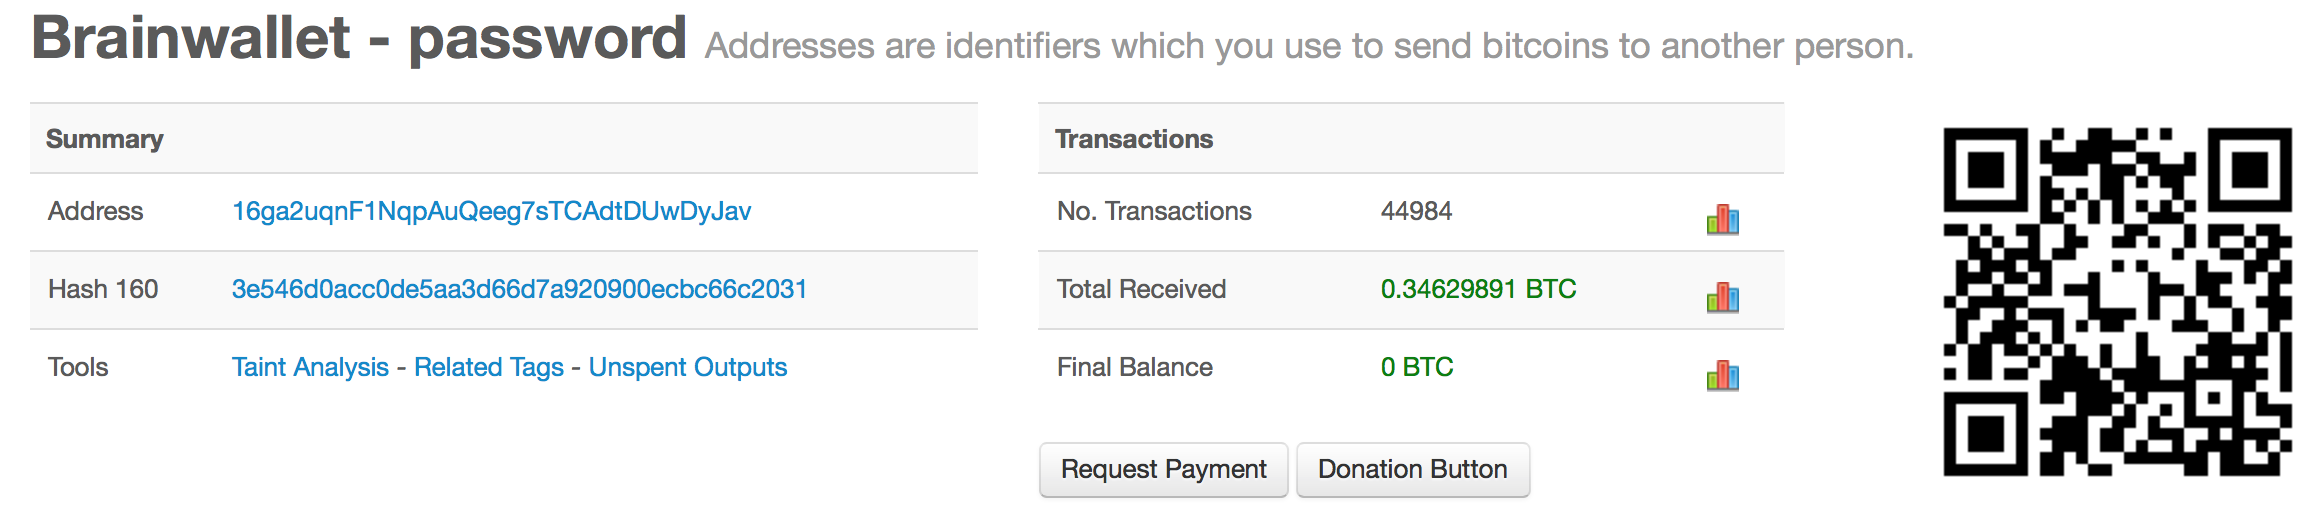
\includegraphics[width=140mm]{./pics/brainwallet-password.png}
	\caption{Brainwallet generated by password ``password''}
	\label{fig:brainwallet_password}
\end{figure}

Brain wallet users are normally urged to use strong passwords or passphrases. Websites provide a brain wallets generation service often using Figure \ref{fig:password_strength} to tell the users what is a strong password. However, this figure is a little bit misleading which makes users feel it is safe to use brain wallets with a passphrase. We have actually cracked quite a few such passphrases. In this thesis we mainly focus on speed optimization of password guessing.

\begin{figure}[h!]
	\centering
	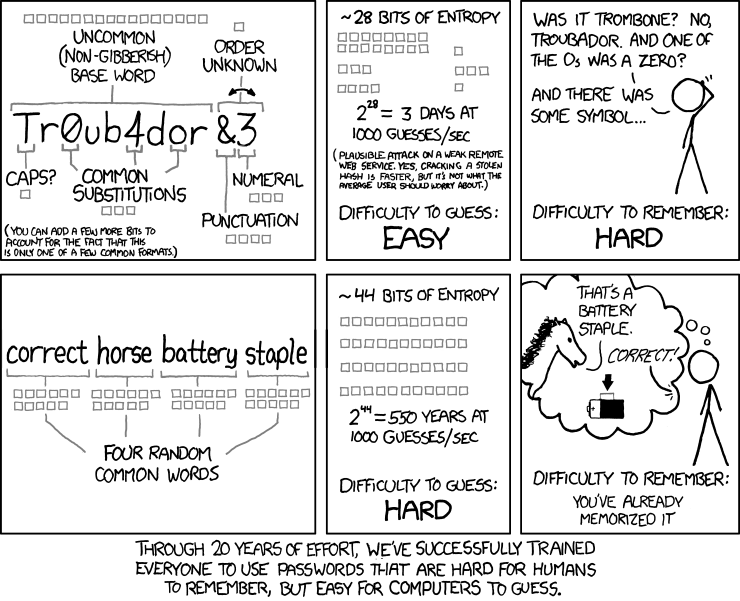
\includegraphics[width=140mm]{./pics/password_strength.png}
	\caption[Password strength comparison between using password and passphrase]{Password strength comparison between using password and passphrase, source: \url{xkcd.com}. This cartoon gives us good advice about how hard it is to guess one user's passwords. But sometimes the speed of guessing can be misleading.}
	\label{fig:password_strength}
\end{figure}

In the next section we will discuss about existing methods of Bitcoin elliptic curve implementation, benchmarking the state-of-art attack and show an improved method of running the attack with much faster speed on a laptop. 
\subsection{Related Work} \label{sec:brainwalletRelatedWork}
We are not the first ones try to crack Bitcoin brain wallets; a lot of other security researchers are doing it. Many victims have found their money stolen and posted it in forums. The first ethical/research brain wallet cracker was announced publicly in a recent hacking conference DEF CON 23 (Aug 2015). Ryan Castellucci, a whitehat hacker, presented his research on cracking brain wallets, and also published his software \cite{RyanDefcon}. Ryan's attack was done on an Intel i7 PC with 4 hyper-threaded cores. The attack speed can reach approximately 16,250 passwords per second on each thread and he had cracked more than 18,000 brain wallet addresses.

The software Ryan has published uses an existing open source secp256k1 Bitcoin elliptic curve implementation mainly written by Pieter Wuille, one of Bitcoin core developers. This implementation is widely used in Bitcoin clients and is considered the current best in terms of code level optimization (detailed benchmarks are given in  table \ref{table:benchmark_msi_affine}).

Later Vasek et al. published their cybercrime analysis results on brain wallets addresses cracked using Ryan's software implementation in FC 2016. Their work was more focused on brain wallets usage measurements and did not try to improve the speed of the attack.

\section{Summary}

